\documentclass[times, utf8, diplomski]{fer}

\usepackage{booktabs}
\usepackage{tikz}
\usepackage{indentfirst}
\usepackage{pgfplots}
\usepackage{graphicx}
\usepackage{caption}
\usepackage{subcaption}
\usepackage{graphicx}

\usetikzlibrary{matrix,calc}

\begin{document}

\thesisnumber{1382}
\title{Image Based Phylogenetic Classification}
\author{Vinko Kodžoman}

\maketitle

% Ispis stranice s napomenom o umetanju izvornika rada. Uklonite naredbu \izvornik ako želite izbaciti tu stranicu.
\izvornik

% Dodavanje zahvale ili prazne stranice. Ako ne želite dodati zahvalu, naredbu ostavite radi prazne stranice.
\zahvala{Thank you...}

\tableofcontents

\chapter{Introduction}
Since the dawn of time, people have tried to explain their surroundings. Life is all around us in many forms, and as such people have tried to categorize it by keen observation, both through its visual and genetic features. Today, it is organised into a taxonomic hierarchy of eight major taxonomic ranks. The number of known species on Earth is in the millions and climbing every year. Great numbers of species make it difficult to classify species based on images and requires domain knowledge. Therefore, an algorithm with the capability to classify species on the filed or from an image using only the image itself could provide great benefits for field researches.

Machine learning allows computers the ability to learn without being explicitly programmed \citep{samuel_studies_1959}. It, together with an increase in available quality data (CIFAR, Imagenet) has yielded great results in the area of deep learning - a class of machine learning algorithms. Deep learning algorithm's accuracy scales with the amount of data used by the algorithm (referenca), that together with the improvements in hardware - mainly general purpose graphic units (GPUs) - has yielded significant performance gains in the last couple of years. One of the most rapidly advancing filed of deep learning is image recognition \citep{krizhevsky_imagenet_2012, simonyan_very_2014, szegedy_going_2015, he_deep_2016} with new neural network architectures being developed almost at a yearly basis, the performance of deep neural networks on image recognition has achieved results previously thought impossible.

In this thesis I propose a solution for a scalable classification of species from images, based on convolution neural networks and recent modern deep learning techniques.

\chapter{Research context}
To fully understand the depth of the image recognition using deep learning, we need a better understand of the underlying algorithms and methods in machine learning, as well as fundamental terms and concepts. In the next section, an introduction of basic terms is given, followed by a detailed explanation of fundamental machine learning algorithms.

\section{Definitions and notation}

\subsection{Image representation}
Matrix is a rectangular array of numbers. It is used because some numbers are naturally represented as matrices. Matrix $A$ with $m$ rows and $n$ columns often written as $m \times n$ has $m*n$ elements and is denoted as $A_{m,n}$. Elements are denoted as $a_{i,j}$ where $i$ and $j$ correspond to the row and column number respectively, as shown in \ref{eq_2d_matrix}. 

\begin{equation} \label{eq_2d_matrix}
A_{m,n} = 
 \begin{bmatrix}
  a_{1,1} & a_{1,2} & \cdots & a_{1,n} \\
  a_{2,1} & a_{2,2} & \cdots & a_{2,n} \\
  \vdots  & \vdots  & \ddots & \vdots  \\
  a_{m,1} & a_{m,2} & \cdots & a_{m,n} 
 \end{bmatrix}
\end{equation}


Each image is represented as a 3 dimensional matrix. One pixel in the image represent a single element in the matrix and as images have multiple channels (RGB) each channel is a 2 dimensional matrix. Image $I$ denoted as $I_{k,m,n}$ where $k\in[0,2]$ represent the channel - red, green or blue - and $m,n\in[0,255]$ represent the pixels in a particular channel as 2 dimensional matrices. Figure \ref{fig:image_matrix} shows a representation of an image as a 3 dimensional matrix where each pixel is denote as $I_{k,m,n}$.


\begin{figure}
\centering
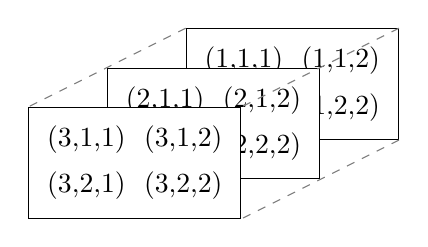
\begin{tikzpicture}
\def\xs{1} %shift in x direction
\def\ys{0.5} %shift in y direction
\def\nm{3} % number of 2d matrices in the 3d matrix
\foreach \x in {1,2,...,\nm}
{

\matrix [draw, % for the rectangle border
         fill=white, % so that it is not transparent
         ampersand replacement=\&] %see explanation
(mm\x)%give the matrix a name
at(-\x * \xs, -\x * \ys) %shift the matrix
{
    \node {(\x,1,1)}; \& \node {(\x,1,2)};\\
    \node {(\x,2,1)}; \& \node {(\x,2,2)};\\
};
}

\draw [dashed,gray](mm1.north west) -- (mm\nm.north west);
\draw [dashed,gray](mm1.north east) -- (mm\nm.north east);
\draw [dashed,gray](mm1.south east) -- (mm\nm.south east);
\end{tikzpicture}
\caption{RGB image with 4 pixels  represented as a 3 dimensional matrix}
\label{fig:image_matrix}
\end{figure}

\subsection{Gradient}
A gradient is a generalization of the derivative in multi-variable space and as such it is represented as a vector. Like the derivative, it represents the slope of the tangent of the graph of the function. Therefore, it points in the direction of the greatest rate of increase of the function. Gradients are widely used in optimization theory as they allow the parameters to shift in a direction which will minimize or maximize a given function. In machine learning the function we want to minimize will be the loss function, which we will define in further chapters in more detail. Gradient of $f$ is denoted as $\nabla{f}$, where every component of $\nabla{f}$ is a partial derivative of $f$, denoted as $\frac{\partial{f}}{\partial{x}}\vec{e}$. Notice that gradient components are vectors denoted as $\vec{e}$. Every vector is written with an horizontal arrow above the letter - $\vec{a}$. The gradient for a $n$ dimensional space is defined in \ref{eq:gradient}.

\begin{equation} \label{eq:gradient}
    \nabla{f}= \frac{\partial{f}}{\partial{x_{1}}}\vec{e_1} + \hdots + 	   \frac{\partial{f}}{\partial{x_{n}}}\vec{e_n}
\end{equation}

\subsection{Activation functions} \label{se:activation_functions}
Machine learning models use nonlinear functions to gain more capacity - expressiveness
. The most popular nonlinear functions are $sigmoid$, $tanh$, $relu$. All nonlinear functions have to have easy to compute gradients, as they are computed on parameters in order to reduce loss as explained above. 
\begin{equation} \label{eq:sigmoid}
	sigmoid(x) = \frac{1}{1 + e^{-x}}
\end{equation}

\begin{equation} \label{eq:tanh}
	tanh(x) = \frac{1 - e^{-2x}}{1 + e^{-2}}
\end{equation}

\begin{equation} \label{eq:relu}
	relu(x) = max(0, x)
\end{equation}
The order of nonlinear functions is given in order of their discoveries. Today relu is used the most, since it solves the problem of vanishing gradients for very deep neural networks, this does not apply to all network types. Recurrent neural networks (RNN) are a class of neural networks that often use $tanh$ as it is better suited for the particular recurrent architecture.

\begin{figure}
    \begin{subfigure}[b]{0.32\textwidth}
        \centering
        \resizebox{\linewidth}{!}{
            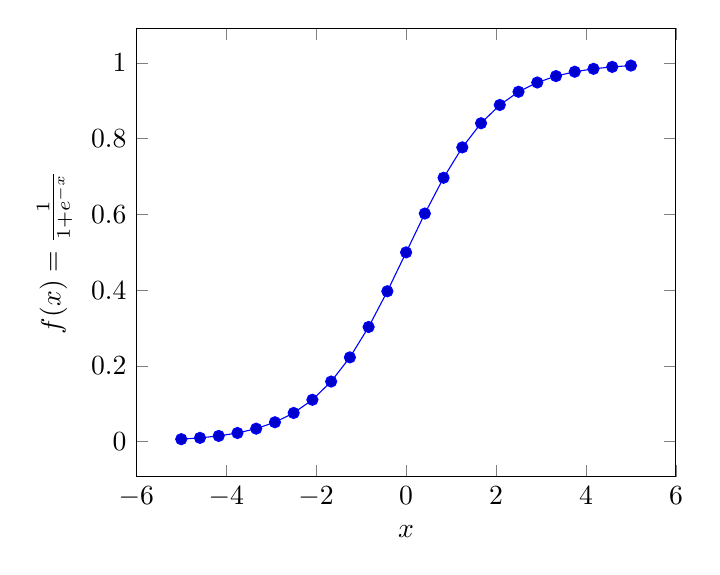
\begin{tikzpicture}
  			\begin{axis}[ 
	  			mark=none,
    			xlabel=$x$,
		    	ylabel={$f(x) = \frac{1}{1 + e^{-x}}$}
		    	] 
	   	 	\addplot {1 /(1 + e^-x)}; 
  			\end{axis}
            \end{tikzpicture}
        }
        \caption{$simgoid$}
        \label{fig:sigmoid}
    \end{subfigure}
    \begin{subfigure}[b]{0.32\textwidth}
    \centering
        \resizebox{\linewidth}{!}{
            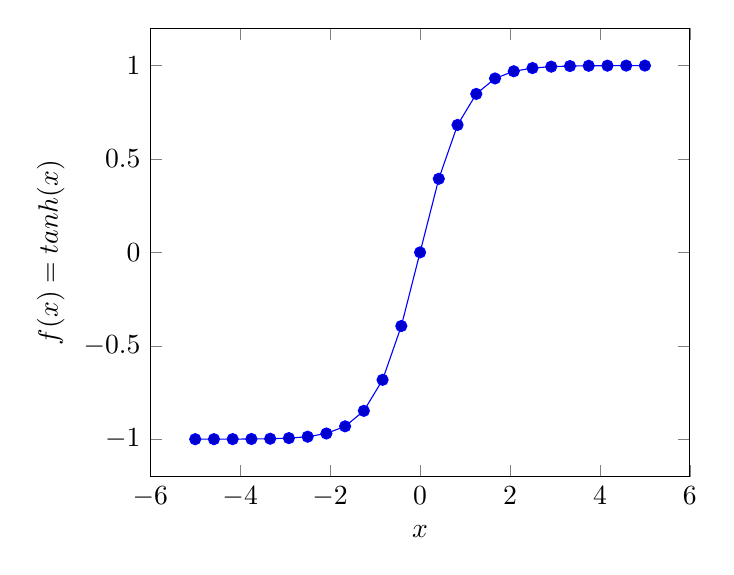
\begin{tikzpicture}
  			\begin{axis}[ 
	  			mark=none,
    			xlabel=$x$,
		    	ylabel={$f(x) = tanh(x)$}
		    	] 
	   	 	\addplot {tanh(x)}; 
  			\end{axis}
            \end{tikzpicture}
        }
        \caption{$tanh$}   
        \label{fig:tanh}
    \end{subfigure}
    \begin{subfigure}[b]{0.32\textwidth}
        \centering
        \resizebox{\linewidth}{!}{
            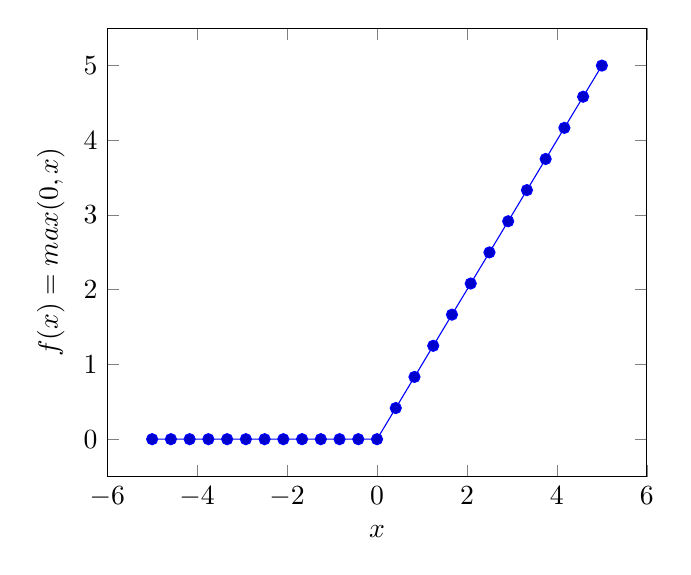
\begin{tikzpicture}
  			\begin{axis}[
  				mark=none,
    			xlabel=$x$,
		    	ylabel={$f(x) = max(0, x)$}
		    	] 
	   	 	\addplot {max(0,x)}; 
  			\end{axis}
            \end{tikzpicture}
        }
        \caption{$relu$}
        \label{fig:relu}
    \end{subfigure}
\caption{Nonliear activation functions} 
\label{fig:subfig1.a.4}
\end{figure}

\subsection{Metrics}
In order to compare different models a set of metrics is employed. Accuracy which gives the accuracy of a model, it is often used on balance datasets (\ref{eq:accuracy}). The problem with unbalanced datasets can be easily explained with a short example. Image having $2$ classes $K=\{dog,cat\}$ and there are a total of $100$ images in the dataset, of which only $2$ are dogs. The model if optimized for accuracy might say the whole dataset is cats which will yield an accuracy of $98\%$. To solve the previous problem, more metrics where introduced for the task of classification; precision (\ref{eq:precision}), recall (\ref{eq:recall}) and F1 score (\ref{eq:f1score}). Precision - positive predictive value - is defined as a fraction of retrieved instances that are relevant. Recall - sensitivity - is a fraction of relevant instances that are retrieved. In order to represent the performance of a model as a single variable F1 score was introduced, it represent a harmonic mean of accuracy and precision.
\begin{equation} \label{eq:accuracy}
	Accuracy = \frac{tp + tn}{tp + tn + fp + fn}
\end{equation}

\begin{equation} \label{eq:precision}
	Precision = \frac{tp}{tp + fp}
\end{equation}

\begin{equation} \label{eq:recall}
	Recall = \frac{tp}{tp + fn}
\end{equation}

\begin{equation} \label{eq:f1score}
	F1 score = 2 * \frac{precision * recall}{precision + recall}
\end{equation}


Classification results are often represented as a confusion matrix, also known as an error matrix.  It is a performance visualisation of a classification model - classifier. To build the classification matrix, conditions of the experiment must be labelled as positive and negative. Using the cats and dogs example from before and marking the cats and a positive and dogs as a negative class. Doing so creates a $2x2$ matrix of actual and predicted values as shown in table \ref{tb:confusion_matrix}.

\begin{table}
\centering
\caption{Confusion matrix}
\label{tb:confusion_matrix}
\begin{tabular}{|c|c|c|}
\hline 
 & \textbf{prediciton} positive & \textbf{prediction} negative \\ 
\hline 
\textbf{actual} positive & True Positive (TP) & False Positive (FP) \\ 
\hline 
\textbf{actual} negative & False Negative (FN) & True Negative (TN) \\ 
\hline 
\end{tabular}
\end{table}

\subsection{Data} \label{se:data}
The input data of the machine learning algorithm is labelled as $D$, and it consists of $X$ and $y_{t}$, where $X$ is one input data (an image in our case) and $y_{t}$ is the true label of the picture - species' name. Written formally the whole input dataset is represented as $D = \{{X}^{\,i},y^{\,i}\}^{N}_{i=1}$, where $i$ is the $i$-th data point and $N$ in the number of data points. Prediction of the algorithm is labelled as $y_{p}$.

The input data set is usually split into two datasets called the \textit{training} a \textit{test} dataset. The training dataset is used to optimize them models parameters while the test data is used to evaluate the model's performance. Sometimes the training dataset is split further into training and \textit{validation} where the validation dataset is used to tune the models \textit{hyperparameters}. Hyperparameters are parameters that do not belong to the model but non the less effect the model's performance. Depth of the neural network is a hyperparameter and will be discussed in later chapters in more detail.


\section{Machine learning}
As said in the Introduction chapter, machine learning allows computers the ability to learn. Giving data to a machine learning algorithm - model - allows it to find patterns within the dataset and to infer. The function that maps the input $X$ to $y_p$ is called a \textit{hypotesis} and is denoted as $h$ (\ref{eq:hypotesis}). The hypotesis $h(X ; \vec{\theta})$ is parametrized with $\vec{\theta}$ - model's parameters.

\begin{equation} \label{eq:hypotesis}
	h(X ; \vec{\theta}) : X \to y
\end{equation}


The model is defined as a set of hypothesises $H$, $h \in H$. Machine learning is the search of the best hypothesis $h$ from the hypothesis space $H$ - typical optimization problem. The algorithm tries to minimize the empirical error function $E(h|D)$ - loss function. The error indicates the accuracy of the hypothesis and is called empirical because it is computed on $D$. Therefore, every machine learning algorithm is defined with the model (\ref{eq:model}), error function (\ref{eq:error_function}) and the optimization method (\ref{eq:optimization_function}).

\begin{equation} \label{eq:model}
	H = \{ h(X ; \vec{\theta}) \}_{\theta}
\end{equation}

\begin{equation} \label{eq:error_function}
	E(h|D) =  \frac{1}{N} \displaystyle\sum_{i=1}^{N} I\{h(X^{\,i}) \neq y^{i}\}
\end{equation}

\begin{equation} \label{eq:optimization_function}
	\theta^{*} = argmin_{\theta} E(\theta | D)
\end{equation}


Machine learning algorithms are divided into groups depending on the task, the groups are classification and regression. Each can be represented as a result of $h(X ; \vec{\theta})$. Classification hypothesis takes the input $X$ and returns a class $k$, example of this method would be image classification. Regression hypothesis takes the input $X$ and returns a number, for example predicting house prices.

\begin{equation} \label{eq:accuracy}
	Regression \equiv h(X ; \vec{\theta}) : X \to y, y \in \mathbb{R}
\end{equation}

\begin{equation} \label{eq:precision}
	Classificatio  \equiv h(X ; \vec{\theta}) : X \to y, y \in K = \{k_{0}, ..., k_{n}\}
\end{equation}

In this chapter we mentioned that machine learning algorithms are trained by minimizing the empirical loss, and in the subsection \ref{se:data} we mentioned the idea of having a training and test set. The goal of the machine learning model is to have good generalization - the ability to work well on never before seen data $X$.


\subsection{Supervised and unsupervised learning}
For the model to be train it needs data $D$ which is defined as $\{{X}^{\,i},y^{\,i}\}^{N}_{i=1}$. Unfortunately, $y$ is not always available. In such cases, the model can still use only $X$ to infer and that is called unsupervised learning. When the model uses both the data points $X$ and labels $y$ it is called supervised learning. Classification and regression are both cases of supervised learning. Cluster analysis or more commonly called clustering is a type of unsupervised learning. In clustering the model tries to group a set of objects in such a way that objects in the same group are more similar based on a cretin metric. The groups are called clusters. Some algorithms need the number of clusters to be predefined, while others discern it by themselves. As the topic of this thesis is classification, in following chapters supervised learning methods will be explained in more detail.

\subsection{Artificial neural network (ANN)}
One of the most interesting models in machine learning, with a diverse set of variations are artificial neural network (ANN). The computational model based on mathematics for neural networks was first introduced in 1943 by Warren McCulloch and Walter Pitts \citep{mcculloch_logical_1943}  called threshold logic. Later on in 1951 a influential paper was published by S. C. Kleene on linking neural networks to finite state automata \citep{kleene_representation_1951}. Artificial neural networks are based on a large collection of small computational unites called neurons (figure\ref{fig:ann_neuron}). The architecture was inspired by axons (\ref{fig:neuron}) from our biological brains. The idea is that even though a single neuron dose not have the capacity to express complicated levels of abstractions - neurons together can. Neurons are connect in order to transfer signals. If a neuron receives a strong enough single it becomes activated and propagates the received single toward his output. Just propagating the single would not be of benefits, as the single would not transform while passing trough the network, therefore non linear activation functions, as explained in subsection \ref{se:activation_functions}, are added to each output of a neuron.

\begin{figure}
  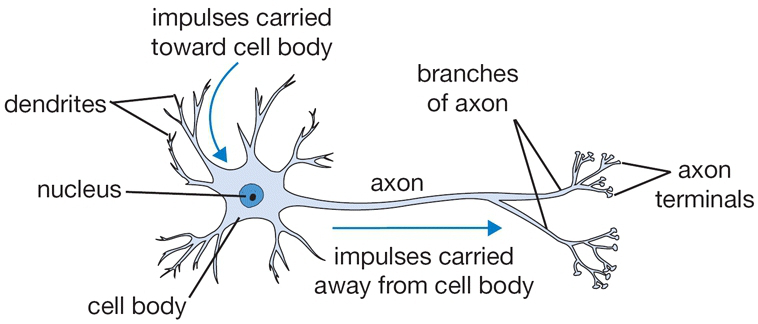
\includegraphics[width=\linewidth]{figures/axon.png}
  \caption{Neuron cell in a biological brain.}
  \label{fig:neuron}
\end{figure}

\begin{figure}
  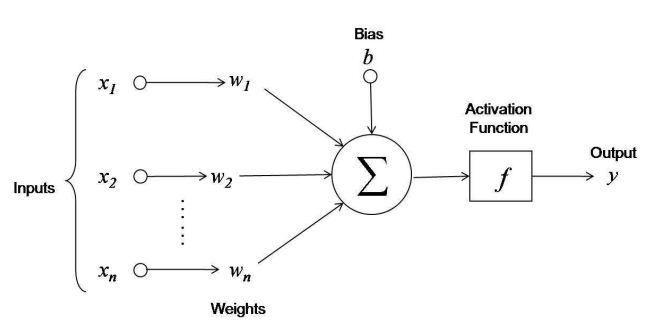
\includegraphics[width=\linewidth]{figures/neuron.jpg}
  \caption{Artificial neuron cell.}
  \label{fig:ann_neuron}
\end{figure}

One of the most popular ANN architectures are feed-forward networks (FFN), sometimes also referred to as fully-connected or dense. They are called feed-forward because the data $X$ enters at on side of the network (the input layer) and exits at the other end (output layer). Neurons are grouped into layers, and layers make an artificial neural network. The first layer is called an input layer, the last layer is called the output layer and everything in between are called hidden layers. The network is called fully-connected because each neuron in the hidden and output layers are connected with ever neuron of the previous layer as seen in figure \ref{fig:ann}.
Each neuron consists of connections, bias and activation function. Each connection has a weight that singles the importance of the connection to the neuron. To get the net output of the neuron we multiple the input vector $\vec{x}$ with the weight vector $\vec{w}$. As the bias (commonly denoted with $w_0$ or $b$), does not have an input of its own we assigned $x_0$ to 1 so we can to a vector multiplication (\ref{eq:neuron_net_output}). To get the final output $y$ of the neuron, the activation function $f$ is applied to the $net$ output, as shown in \ref{eq:neuron_output}). computational model of the artificial neuron can bee seen in the figure \ref{fig:ann_neuron}.

\begin{equation}
	\label{eq:neuron_net_output}
	net = 1*w_0 + w_1*x_1 + ... + w_n*x_n = \vec{x} * \vec{w}
\end{equation}

\begin{equation}
	\label{eq:neuron_output}
	y = f(net) = f(\vec{x}*\vec{w})
\end{equation}

\begin{figure}
  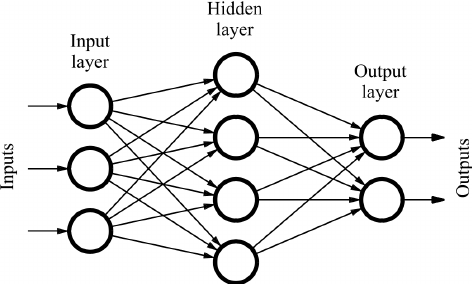
\includegraphics[width=\linewidth]{figures/ann.png}
  \caption{Feed-forward neural network}
  \label{fig:ann}
\end{figure}

Artificial neuron networks have the ability to adjust their capacity to the task. Adjusting the number of neurons in a single layer, the number of hidden layers or the type of activation function used in each neuron affects the capacity of the ANN. Such flexibility also leads to a broad number of architectures, and there is no clear way to determine which one suits best. It is often left to the user to test a broad variety of architectures. Looking at the figure \ref{fig:ann} we can see that the number of neurons in the input layer matches the input size, this is true also for the output layer. There fore when designing an ANN the size of input and output layers are determined by the task and the hidden layer by the user.


\section{Deep learning}
GPUs

\subsection{Feedforward Neural Networks}
\subsection{Convolutional Neural Networks}
\subsection{Backpropagation}
\subsection{Vanishing Gradient}
\subsection{Batch Normalization}
\subsection{Data Augmentation}


\chapter{TaxNet}
Let's hope it is any good.
\section{Implementation}

\chapter{Dataset}
\subsection{ImageNet}

\chapter{Results}
Graphs graphs graphs...

\chapter{Conclusion}
Zaključak.

\bibliographystyle{fer}
\bibliography{master_thesis}


\begin{sazetak}
Sažetak na hrvatskom jeziku.

\kljucnerijeci{Ključne riječi, odvojene zarezima.}
\end{sazetak}

% TODO: Navedite naslov na engleskom jeziku.
\engtitle{Title}
\begin{abstract}
Abstract.

\keywords{Keywords.}
\end{abstract}

\end{document}